\documentclass{standalone}
\usepackage{tikz}
\usepackage{amsmath}
\renewcommand{\familydefault}{\sfdefault}


\begin{document}
\pagestyle{empty}
% \definecolor{colorsrc}{rgb}{0.36, 0.54, 0.66}

% \definecolor{colornan}{rgb}{0.5, 0.5, 0.5}
% \definecolor{colornan}{rgb}{0.43, 0.21, 0.1}
% \definecolor{auburn}{rgb}{0.43, 0.21, 0.1}
% \definecolor{colorwnd2}{rgb}{1, .44, .37}
\definecolor{colorlcksvd}{rgb}{0.91, 0.84, 0.42}
\definecolor{colorlcksvdd}{rgb}{0.8, 0.0, 0.1}
\definecolor{colorlcksvd}{rgb}{1, 0.56, 0.0}
% \definecolor{colornan}{rgb}{0, 0.8, 0.0}
% \definecolor{colorsrc}{rgb}{0.5, 1, 0}
% \definecolor{colorfdd}{rgb}{0.6, 0.4, 0.8}
% \definecolor{colorfdd}{rgb}{0.93, 0.53, 0.18}
\definecolor{colorfddl}{rgb}{0.44, 0.16, 0.39}
\definecolor{colordlsi}{rgb}{0.55, 0.71, 0.0}
% \definecolor{colorlck}{rgb}{0.43, 0.21, 0.1}
% \definecolor{colorlck}{rgb}{0.89, 0.82, 0.04}
% \definecolor{colorlck}{rgb}{0.03, 0.27, 0.49}
\definecolor{colorcopar}{rgb}{0.9, .0, 0}
% \definecolor{colorlrsd}{rgb}{0.72, 0.53, 0.04}
\definecolor{colorjdl}{rgb}{0.0, 0.55, 0.55}
\definecolor{colordlr}{rgb}{0.0, 0.55, 0.55}
\definecolor{colorlrsdl}{rgb}{0.0, 0.2, 1.0} % blue
% \definecolor{colorlck}{rgb}{0.5, 0.5, 0.0}
% \definecolor{colorlck}{rgb}{0.0, 0.42, 0.24}
\definecolor{colorlck}{rgb}{0.0, 0.9, 0.9}
\definecolor{pinegreen}{rgb}{0.0, 0.47, 0.44}

\def\myaddplotlrsdl{\addplot+[thick, colorlrsdl, solid, mark = square*, mark size=1.4, mark options={colorlrsdl}]}
\def\myaddplotfddl{\addplot+[thick, colorfddl, mark = diamond*, mark size=1.4, mark options={colorfddl}]}
\def\myaddplotlcksvd{\addplot+[thick, colorlcksvd, mark = x, mark size=1.8, mark options={colorlcksvd}]}
\def\myaddplotlcksvdd{\addplot+[thick, green, mark = triangle, mark size=1.4, mark options={green}]}
\def\myaddplotdlsi{\addplot+[thick, colordlsi, mark = *, mark size=1.4, mark options={fill = white}]}
\def\myaddplotsrc{\addplot+[thick, colorsrc, mark = square, mark size=1.4, mark options={colorsrc}]}
\def\myaddplotcopar{\addplot+[thick, colorcopar, solid, mark = *, mark size=1.4, mark options={colorcopar}]}
\def\myaddplotjdl{\addplot+[thick, pinegreen, solid, mark = diamond*, mark size=1.4, mark options={pinegreen}]}
\def\myaddplotdlr{\addplot+[thick, cyan, solid, dashed, mark = triangle*, mark size=1.4, mark options={cyan}]}


% \def\myaddplotcopar{\addplot+[colorcopar, mark = square*, mark options={colorcopar}]}
% \def\myaddplotdfd{\addplot+[colordfd,  mark options={colordfd}]}
% \def\myaddplotfdd{\addplot+[colorfdd,  mark options={colorfdd}]}
% \def\myaddplotlck{\addplot+[colorlck,  mark options={colorlck}]}
% \def\myaddplotnan{\addplot+[colornan,  mark options={colornan}]}
% \def\myaddplotwnd{\addplot+[colorwnd,  mark options={colorwnd}]}
% \def\wnd{{black,fill=colorwnd}}

\def\x{{\mathbf x}}
\def\L{{\cal L}}

\newcommand{\vect}[1]{\mathbf{#1}}

\newcommand{\mat}[1]{\mathbf{#1}}
\newcommand{\abs}[1]{\left|#1\right|}
\newcommand{\norm}[1]{\left\|#1\right\|}
% \newcommand{\R}{\mathbb{R}}
\newcommand{\Z}{\mathbb{Z}}
\newcommand{\tb}{\textbf}


\def\bmt{\left[\begin{matrix}}
\def\dpcm{$\square$}
\def\emt{\end{matrix}\right]}
% \def\proof{\underline{Proof:}\\}
\def\dpcm{$\square$}
\def\half{\frac{1}{2}}
\def\imply{\Rightarrow}
\def\foralli{\forall i = 1, 2, \dots, n}
\def\im{\mathrm{im}}
\def\ker{\mathrm{ker}}
\def\eqv{\Leftrightarrow}
\def\tcg{\textcolor{newgreen}}
\def\mb{\mathbf}
\def\tb{\textbf}
\def\mb {\mathbf}
\def\mc {\mathcal}
\def\tcb{\textcolor{blue}}
\def\tcg{\textcolor{green}}
\def\tcr{\textcolor{red}}
\def\tcgr{\textcolor{gray}}
\def\bx{\mathbf{x}}
% \def\bW{\mathbf{W}}
\def\ba{\mathbf{a}}
\def\bb{\mathbf{b}}
\def\bc{\mathbf{c}}
\def\bd{\mathbf{d}}
\def\be{\mathbf{e}}
\def\fb{\mathbf{f}}
\def\bg{\mathbf{g}}
\def\bh{\mathbf{h}}
\def\bm{\mathbf{m}}
\def\M{\mathcal{M}}
\def\bp{\mathbf{p}}
\def\bq{\mathbf{q}}
\def\bs{\mathbf{x}}
\def\bu{\mathbf{u}}
\def\bv{\mathbf{v}}
\def\by{\mathbf{y}}
\def\bz{\mathbf{z}}
\def\and{\text{~and~}}
\def\barN{\bar{N}}
\def\barNi{\bar{N}_i}
\def\trace{\textrm{trace}}
\def\etal{\textit{et al.}}
\def\R{\mathbb{R}}

\def\bzeros{\mathbf{0}}

\def\bA{\mathbf{A}}
\def\bB{\mathbf{B}}
\def\bD{\mathbf{D}}
\def\bE{\mathbf{E}}
\def\Fb{\mathbf{F}}
\def\bG{\mathbf{G}}
\def\bL{\mathbf{L}}
\def\bH{\mathbf{H}}
\def\bI{\mathbf{I}}
\def\bJ{\mathbf{J}}
\def\bM{\mathbf{M}}
\def\bN{\mathbf{N}}
\def\bP{\mathbf{P}}
\def\bQ{\mathbf{Q}}
\def\bR{\mathbf{R}}
\def\bS{\mathbf{S}}
\def\bU{\mathbf{U}}
\def\bV{\mathbf{V}}
\def\bW{\mathbf{W}}
\def\bX{\mathbf{X}}

\def\bY{\mathbf{Y}}
\def\bZ{\mathbf{Z}}
\def\rank{\text{rank}}
\def\bDi{\mathbf{D}_i}
% \def\bSi{\mathbf{X}_i}
\def\bXi{\mathbf{X}_i}
% \def\bSi{\mathbf{X}_i}
\def\barX{\bar{\mathbf{X}}}
\def\barD{\bar{\mathbf{D}}}
\def\barX{\bar{\mathbf{X}}}
\def\barXi{\bar{\mathbf{X}}_i}
\def\barDi{\bar{\mathbf{D}}_i}
\def\barXi{\bar{\mathbf{X}}_i}
\def\bW{\mathbf{W}}
\def\bw{\mathbf{w}}

\def\la{\langle}
\def\ra{\rangle}

\def\bDc{\bD_{0}}
\def\bXc{\bX^{0}}
\def\mM{\mathcal{M}}
\def\wt{\widetilde}

\def\bbX{\lbar{\bX}}        
\def\bbx{\lbar{\bx}}        
\def\bbY{\lbar{\bY}}        
\def\bbD{\lbar{\bD}}  

%% ================== block: Slide footnotes ==========================
\def\footnoteSRC{\setcounter{footnote}{3}\footnote[frame]{\tiny J. Wright et al., Robust face recognition via sparse representation, IEEE TPAMI, 2009}}
\def\footnoteLLC{\setcounter{footnote}{4}\footnote[frame]{\tiny  H. Zhang et. al., Locality-constrained linear coding for image classification, CPVR 2010}}
\def\footnoteJSRC{\setcounter{footnote}{5}\footnote[frame]{\tiny  Yen, Multi-View Automatic Target Recognition using Joint Sparse Representation, Aerospace and Electronic Sys. 2012}}
\def\footnoteJDSRC{\setcounter{footnote}{6}\footnote[frame]{\tiny  J. Wang et. al., Joint dynamic sparse representation for multi-view face recognition,  PR 2012}}
\def\footnoteSHIRC{\setcounter{footnote}{7}\footnote[frame]{\tiny U. Srinivas et. al., Simultaneous sparsity model for histopathological image representation and classification, TMI 2014}}
\def\footnoteKSVD{\setcounter{footnote}{8}\footnote[frame]{\tiny  M. Elad et. al., K -SVD: An Algorithm for Designing Overcomplete Dictionaries for Sparse Representation, TSP 2006 }}
\def\footnoteODL{\setcounter{footnote}{9}\footnote[frame]{\tiny J. Mairal et. al., Online learning for matrix factorization and sparse coding, JMLR 2010}}
\def\footnoteDKSVD{\setcounter{footnote}{10}\footnote[frame]{\tiny  Q. Zhang, B. Li, Discriminative K-SVD for dictionary learning in face recognition, CVPR 2010 }}

\def\footnoteLCKSVD{\setcounter{footnote}{11}\footnote[frame]{\tiny  Z. Jiang et. al., Label consistent K-SVD: Learning a discriminative dictionary for recognition, TPAMI 2013}}
\def\footnoteFDDL{\setcounter{footnote}{12}\footnote[frame]{\tiny  M. Yang et. al., Fisher discrimination dictionary learning for sparse representation, ICCV 2011, IJCV 2014 }}
\def\footnoteDLR{\setcounter{footnote}{20}\footnote[frame]{\tiny  L. Li et. al., Learning low-rank and discriminative dictionary for image classification, Image and Vision Computing, 2014}}
\def\footnoteOMP{\setcounter{footnote}{13}\footnote[frame]{\tiny  Tropp et. al., Signal recovery from random measurements via orthogonal matching pursuit,  IEEE Transactions on Information Theory 2007}}
\def\footnoteNANDITA{\setcounter{footnote}{14}\footnote[frame]{\tiny N. Nayak et. al., Classification of tumor histopathology via sparse feature learning, ISBI 2013}}
\def\footnoteWNDCHARM{\setcounter{footnote}{15}\footnote[frame]{\tiny L. Shamir et. al., WNDCHARM--an open source utility for biological image analysis,  Source Code Biol. Med., 2008}}

\def\footnoteDFDLTMI{\setcounter{footnote}{16}\footnote[frame]{\tiny  \tcr{T. Vu} et. al., Histopathological Image Classification using Discriminative Feature-oriented Dictionary Learning, TMI 2015}}
\def\footnoteADMM{\setcounter{footnote}{17}\footnote[frame]{\tiny S. Boyd et. al., Distributed Optimization and Statistical Learning via the Alternating Direction Method of Multipliers, Foundations and Trends in Machine Learning, 2011}}
\def\footnoteFISTA{\setcounter{footnote}{18}\footnote[frame]{\tiny A. Beck et. al., A fast iterative shrinkage-thresholding algorithm for linear inverse problems, SIAM journal on Imaging sciences, 2009}}
\def\footnoteHojjatJPI{\setcounter{footnote}{19}\footnote[frame]{\tiny H. Mousavi \etal, Automated discrimination of lower and higher grade gliomas based on histopathological image analysis, JPI, 2015}}
% \def\footnote
% \def\footnoteDLSI{\setcounter{footnote}{3}\footnote[frame]{\tiny  I. Ramirez et. al., IEEE Computer Vision and Pattern Recognition (CVPR), 2010 }}






\def\footnotea{\setcounter{footnote}{3}\footnote[frame]{\tiny  H. Chang et. al., IEEE Transactions on Medical Imaging (TMI), 2013}}
\def\footnoteb{\setcounter{footnote}{4}\footnote[frame]{\tiny E. Ozdemir et. al., IEEE Transactions on Medical Imaging (TMI), 2013}}
\def\footnotec{\setcounter{footnote}{5}\footnote[frame]{\tiny M. Murat Dundar et. al., IEEE Transactions on Biomedical Engineering (TBME), 2011}}

\def\footnoteGDDL{\setcounter{footnote}{21}\footnote[frame]{\tiny  Suo et. al., Structured dictionary learning for classification, submitted to TSP 2014}}
\def\footnoteDLCORPA{\setcounter{footnote}{22}\footnote[frame]{\tiny S. Kong et. al., ECCV 2012}}
\def\footnoteDDLPC{\setcounter{footnote}{23}\footnote[frame]{\tiny  Guo et. al., ACCV 2012}}
\def\footnoteLPDDL{\setcounter{footnote}{24}\footnote[frame]{\tiny  Haghiri et. al., ICIP 2014}}
\def\footnoteDLSI{\setcounter{footnote}{25}\footnote[frame]{\tiny  Ramirez et. al., Classification and clustering via dictionary learning with structured incoherence and shared features, CVPR 2010}}
\def\footnoteDFDL{\setcounter{footnote}{26}\footnote[frame]{\tiny  T. Vu et. al., ISBI 2015}}
\def\footnoteDLRDSR{\setcounter{footnote}{27}\footnote[frame]{\tiny L. Ma et. al., CVPR 2012}}
\def\footnoteTDDL{\setcounter{footnote}{28}\footnote[frame]{\tiny J. Mairal et. al., ``Task-driven dictionary learning'', TPAMI, 2012}}
\def\footnoteTDDLLP{\setcounter{footnote}{29}\footnote[frame]{\tiny X. Sun, N. Nasrabadi, T. Tran, ``Task-driven dictionary learning for hyperspectral image classification with structured sparsity constraints'', TGRS, 2015}}
\def\footnoteJohn{\setcounter{footnote}{30}\footnote[frame]{\tiny J. Mckay, V. Monga \etal, Pose corrected sparsity for robust SONAR ATR, IGRSS, 2016}}



\def\diag{\text{diag}}


%% ------------------end of block: Slide footnotes ----------------------------



\newcommand{\myFormA}[1]{\bmt #1 & \bzeros & \dots & \bzeros \\ \bzeros & #1 & \dots & \bzeros \\ \dots & \dots & \dots & \dots \\ \bzeros & \bzeros & \dots & #1  \emt}
\newcommand{\myFormB}[1]{\bmt #1 & #1 & \dots & #1 \\ #1 & #1 & \dots & #1 \\ \dots & \dots & \dots & \dots \\ #1 & #1 & \dots & #1  \emt}

        
%% ========= long bar notation ==============================
\makeatletter
\newsavebox\myboxA
\newsavebox\myboxB
\newlength\mylenA
\newcommand*\lbar[2][.75]{%
    \sbox{\myboxA}{$\m@th#2$}%
    \setbox\myboxB\null% Phantom box
    \ht\myboxB=\ht\myboxA%
    \dp\myboxB=\dp\myboxA%
    \wd\myboxB=#1\wd\myboxA% Scale phantom
    \sbox\myboxB{$\m@th\overline{\copy\myboxB}$}%  Overlined phantom
    \setlength\mylenA{\the\wd\myboxA}%   calc width diff
    \addtolength\mylenA{-\the\wd\myboxB}%
    \ifdim\wd\myboxB<\wd\myboxA%
       \rlap{\hskip 0.5\mylenA\usebox\myboxB}{\usebox\myboxA}%
    \else
        \hskip -0.3\mylenA\rlap{\usebox\myboxA}{\hskip 0.3\mylenA\usebox\myboxB}%
    \fi}
\makeatother

\def\lbD{\lbar{\bD}}
\def\lbY{\lbar{\bY}}
\def\lbX{\lbar{\bX}}
% \def\lbX{\overline{\mathbf{X}}}
% \def\lbY{\overline{\mathbf{Y}}}
\def\layersep{2.5cm}
\tikzset{dist/.style={path picture= {
    \begin{scope}[x=1pt,y=10pt]
      % \draw plot[domain=-6:6] (\x,{1/(1 + exp(-\x))-0.5});
      % \draw plot[domain=0:6] (\x,.5);
      % \draw plot[domain=-6:0] (\x,-.5);
      % \draw (0, -.5) -- (0, .5);
        \def\a{5}
      \draw [blue] (-\a, -.5) --  (\a, .5);
      % \draw [thin] (-1.1*\a, 0) -- (1.2*\a, 0);
      % \draw [thin] (0, -.7) -- (0, .8);
    \end{scope}
    }
  }
}
\tikzstyle{every pin edge}=[shorten <=1pt]
\tikzstyle{neuron}=[circle,fill=black!25,minimum size=17pt,inner sep=0pt]
\tikzstyle{input neuron}=[neuron, thick, draw = black, fill=green!40]
\tikzstyle{output neuron}=[neuron,thick, draw = black, fill=red!40]
\tikzstyle{linear neuron}=[output neuron, dist]
\tikzstyle{hidden neuron}=[neuron, thick, draw = black, fill=blue!40]
\tikzstyle{annot} = [text width=4em, text centered]
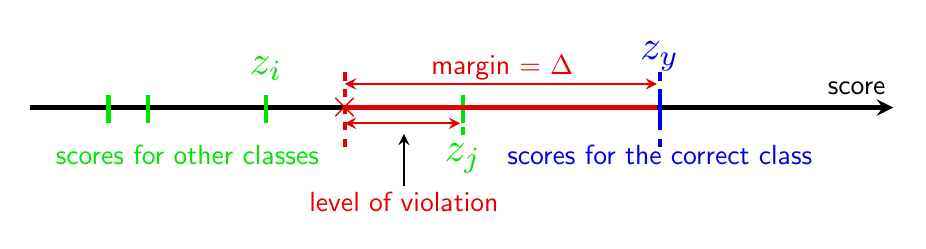
\begin{tikzpicture}[shorten >=1pt,draw=black,thick, node distance=\layersep, >= stealth]

    \draw [->, ultra thick] (-1, 0) -- (10, 0);
    \node at (9.5, 0.25) {score};
    \foreach \x in {0, 0.5, 2, 4.5} {
        \draw [ultra thick, green!90!black] (\x, -.2) -- (\x, .2);        
    }

    \node at (2, .5) [scale = 1.5, green!90!black] {$z_i$};
    \node at (7, .65) [scale = 1.5, blue!90!black] {$z_y$};
    \node at (4.5, -.65) [scale = 1.5, green!90!black] {$z_j$};


    \draw [ultra thick, blue!90!black, dashed] (7, -.5) -- (7,  .5);
    \draw [ultra thick, blue!90!black] (7, -.2) -- (7,  .2);
    \draw [ultra thick, red!90!black, dashed] (3, -.5) -- (3,  .5);
    \draw [ultra thick, green!90!black, dashed] (4.5, -.35) -- (4.5,  .2);

    \node at (1, -.6) [align = center, green!90!black] {scores for other classes};
    \node at (7, -.6) [align = center, blue!90!black] {scores for the correct class};

    \draw [ultra thick, red!90!black] (3, 0) -- (7, 0);

    \draw [<->, thick, red!90!black] (3, .3) -- (7, .3);
    \draw [<->, thick, red!90!black] (3, -.2) -- (4.5, -.2);
    \node at (5, .5) [align = center, red!90!black] {margin = $\Delta$};

    \node at (3, 0) [red!90!black] {\Large \bf $\times$};

    \node at (3.75, -1.2) [red!90!black] {level of violation};

    \draw [->] (3.75, -1) -- (3.75, -.3);
\end{tikzpicture}
% End of code
\end{document}
